\documentclass[12pt,titlepage]{article}
%\usepackage[spanish]{babel}
%\usepackage[utf8]{inputenc}
%\usepackage[utf8]{inputenc}
\usepackage{amsmath}
\usepackage{amssymb}
\usepackage{graphicx}
%\usepackage{caratula}
\usepackage{float}
\usepackage{subfigure}
\usepackage{wrapfig}
\usepackage{listings}
\usepackage{ulem}
%\usepackage{float}
\usepackage{xunicode,xltxtra,url,parskip}
\usepackage{fontspec}
\defaultfontfeatures{Mapping=tex-text}
\setmainfont[SmallCapsFont = Fontin SmallCaps]{Fontin}
%\lstset{language=C,basicstyle=\small\tt,keywordstyle=\bf,tabsize=3,breaklines=true,linewidth=16cm,postbreak={\mbox{$\rightsquigarrow$}},prebreak={\mbox{$\rightsquigarrow$}}}
\lstset{language=SQL,basicstyle=\small\tt,keywordstyle=\bf,tabsize=3,breaklines=true,linewidth=16cm,postbreak={\mbox{$\rightsquigarrow$}},prebreak={\mbox{$\rightsquigarrow$}}}

%\usepackage{a4wide}
%\usepackage{amssymb}
%\usepackage{amsmath}
 \usepackage{enumerate}
 \parindent = 12 pt
 \parskip = 12 pt
%\usepackage[width=15.5cm, left=3cm, top=2.5cm, height= 24.5cm]{geometry}

\usepackage{color}
\usepackage{url}
\definecolor{lnk}{rgb}{0,0,0.4}
\usepackage[colorlinks=true,linkcolor=lnk,citecolor=blue,urlcolor=blue]{hyperref}

\newcommand{\func}[2]{\texttt{#1}(#2) :}
\newcommand{\tab}{\hspace*{2em}}
\newcommand{\FOR}{\textbf{for }}
\newcommand{\TO}{\textbf{ to }}
\newcommand{\IF}{\textbf{if }}
\newcommand{\WHILE}{\textbf{while }}
\newcommand{\THEN}{\textbf{then }}
\newcommand{\ELSE}{\textbf{else }}
\newcommand{\RET}{\textbf{return }}
\newcommand{\MOD}{\textbf{ \% }}
\newcommand{\OR}{\textbf{ or }}
\newcommand{\NOT}{\textbf{ not }}
\newcommand{\tOde}[1]{\tab \small{\mathcal{O}($#1$)}}
\newcommand{\Ode}[1]{\ensuremath{\small{\mathcal{O}\left(#1\right)}}}
\newcommand{\VSP}{\vspace*{3em}}
\newcommand{\Pa}{\vspace{5mm}}
\newenvironment{pseudo}{\noindent\begin{tabular}{ll}}{\end{tabular}\VSP}

\newenvironment{while}{\WHILE \\ \setlength{\leftmargin}{0em} }{}

\newcommand{\iif}{\Leftrightarrow}
\newcommand{\gra}[1]{\noindent\includegraphics[scale=.70]{#1}\\}
\newcommand{\gras}[2]{\noindent\includegraphics[scale=#2]{#1}\\}
\newcommand{\grasize}[2]{\noindent\includegraphics[width=#2]{#1}\\}
\newcommand{\gram}[1]{\noindent\includegraphics[scale=.50]{#1}}
\newcommand{\dirmail}[1]{\normalsize{\texttt{#1}}}
\newenvironment{usection}[1]{\newpage\begin{section}*{#1}	\addcontentsline{toc}{section}{#1}}{\end{section}}
\newenvironment{ucsection}[1]{\newpage\begin{section}*{#1}	\addcontentsline{toc}{section}{#1}}{\end{section}}
\newenvironment{usubsection}[1]{\begin{subsection}*{#1}	\addcontentsline{toc}{subsection}{#1}}{\end{subsection}}

\newenvironment{mr}[1]{\noindent\begin{minipage}[t]{.5\linewidth}\vspace{0pt}\begin{tabular}{|l|}\hline{\textbf{\large #1}}\\ \hline\hline}{\hline\end{tabular}\vspace{.5cm}\end{minipage}}
\newcommand{\PRI}[1]{\uline{#1}}
\newcommand{\FORE}[1]{\uwave{#1}}
\newcommand{\PRIFOR}[1]{\PRI{\FORE{#1}}}


\newcommand{\superref}[1]{\textsuperscript{\ref{#1}}}

\addtolength{\topmargin}{-2cm}
\addtolength{\textheight}{3cm}

\begin{document}

\begin{titlepage}
\begin{center}
{\textbf{Universidad de Buenos Aires}\\Facultad de Ciencias Exactas y Naturales}

\vspace{1.5cm}

\begin{tabular}{r}
{\Large \bfseries Bases de Datos}\\
\hline
\textsc{\small 1er cuatrimestre 2011}\\
\end{tabular}
\vspace{2cm}

\begin{tabular}{l}
{\large TP1}\\
\textbf{\Huge DER, MR, SQL}\\
\end{tabular}

\vspace{1cm}

%\begin{minipage}[b]{0.7\linewidth}
%\begin{tabular}{l}
%\textbf{Abstract}\\
%{In this document we analyze the differences of the methods PSSM (Position-Specific Scoring Matrix) and ANN (Artificial neural networks) for Peptide MHC binding predictions.}\\
%\end{tabular}
%\end{minipage}

\vspace{1cm}

\begin{tabular}{lr}
Mariano Bianchi & \texttt{marianobianchi08@gmail.com}\\
Pablo Brusco & \texttt{pablo.brusco@gmail.com}\\
Julian Dondero & \texttt{juliandondero@gmail.com}\\
Ezequiel Castellano & \texttt{ezequiel.castellano@gmail.com}\\
Kevin Allekotte & \texttt{kevinalle@gmail.com}\\
\end{tabular}

\vspace{2cm}

{\large Mayo 2011}

\end{center}
\end{titlepage}
\protect\setcounter{tocdepth}{1}
%\tableofcontents
%\newpage

	\begin{ucsection}{DER}
		\begin{figure}[ht!]
			\noindent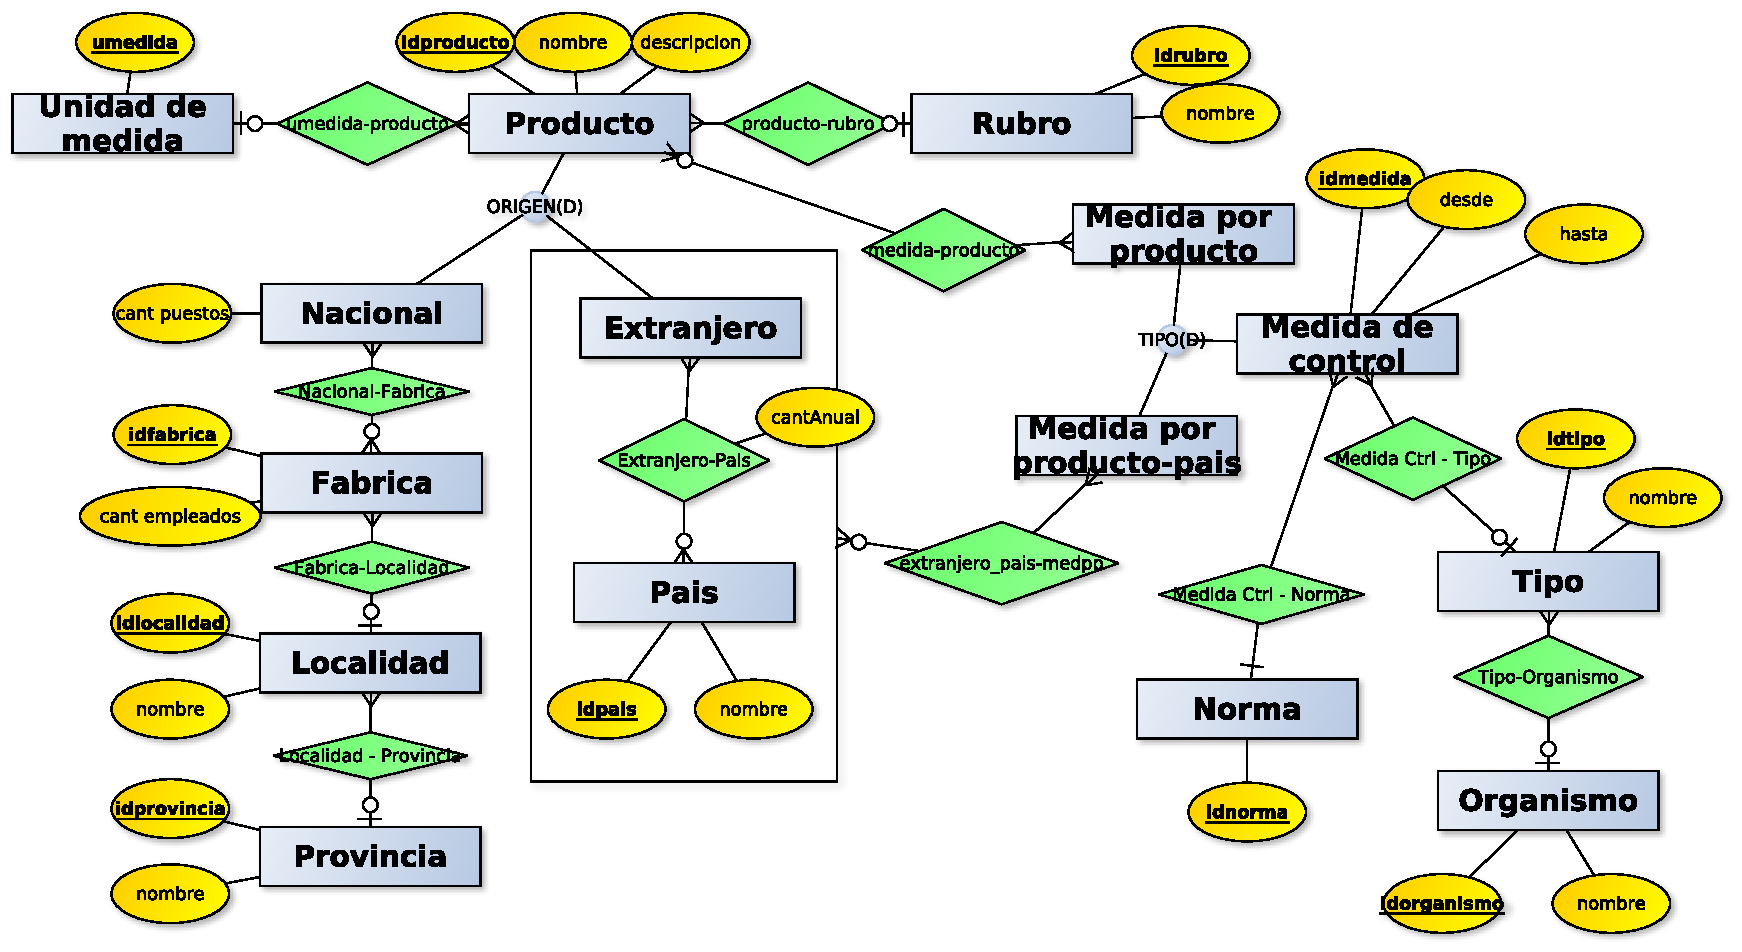
\includegraphics[angle=90,height=20cm]{der.pdf}
			\label{fig:der}
		\end{figure}
		
		\newpage
		\begin{usubsection}{Decisiones tomadas}
		\begin{enumerate}
			\item Todos los productos tienen una Unidad de Medida asociada.
			\item Pueden existir Unidades de Medida, sin Productos asociados.
			\item Pueden existir Rubros, sin Productos asociados.
			\item Pueden existir Fábricas sin Productos asociados.
			\item Pueden existir Localidades sin Fábricas asociadas.
			\item Pueden existir Provincias sin Localidades.
			\item Pueden existir Países sin Productos asociados.
			\item Pueden haber Productos, sin Medidas de Control asociadas.
			\item No pueden existir Medidas de Control, sin Normas asociadas.
			\item No pueden existir Normas sin Medidas de Control asociadas.
			\item Pueden haber Tipos sin Medidas de control asociadas.
			\begin{enumerate}
				{\footnotesize \item \textbf{Obs:} No habría Medidas de Control para todo Tipo, con lo cual no existirian Productos con Medidas de control de todos los tipos.} 
			\end{enumerate}
			\item Un Organismo puede controlar varios Tipos de Medidas de Control.
			\item Un Tipo de Medida de Control es controlado por un solo Organismo.
			\item Pueden existir Organismos sin Tipos de Medidas de Control asociados.
			\item Todo Tipo de Medida de Control tiene un Organismo que lo controla.
			\item Decidimos no modelar la parte de auditoría del problema, consideramos que no pertenecía directamente al mismo y que era mejor no incluirlo en el DER. 
		\end{enumerate}
		\end{usubsection}
	\end{ucsection}
	
	\begin{ucsection}{MR}
		\begin{mr}{pais}\PRI{idpais}\\nombre\\\end{mr}
		\begin{mr}{fabrica}\PRI{idfabrica}\\cantempleados\\\FORE{idlocalidad}\\\end{mr}
		\begin{mr}{localidad}\PRI{idlocalidad}\\nombre\\\FORE{idprovincia}\\\end{mr}
		\begin{mr}{provincia}\PRI{idprovincia}\\nombre\\\end{mr}
		\begin{mr}{rubro}\PRI{idrubro}\\nombre\\\end{mr}
		\begin{mr}{tipo}\PRI{idtipo}\\nombre\\\FORE{idorganismo}\\\end{mr}
		\begin{mr}{organismo}\PRI{idorganismo}\\nombre\\\end{mr}
		\begin{mr}{norma}\PRI{idnorma}\\\end{mr}
		\begin{mr}{udemedida}\PRI{umedida}\\\end{mr}
		\begin{mr}{producto}\PRI{idproducto}\\nombre\\descripcion\\\FORE{umedida}\\origen\\\FORE{idrubro}\\\end{mr}
		\begin{mr}{medida}\PRI{idmedida}\\\FORE{idnorma}\\\FORE{idtipo}\\tipo\\desde\\hasta\\\end{mr}
		\begin{mr}{prod\_extranjero-pais}\PRIFOR{idproducto}\\\PRIFOR{idpais}\\cantanual\\\end{mr}
		\begin{mr}{prod\_nacional\_fabrica}\PRIFOR{idproducto}\\\PRIFOR{idfabrica}\\\end{mr}
		\begin{mr}{producto\_extranjero}\PRIFOR{idproducto}\\\end{mr}
		\begin{mr}{producto\_naciona}\PRIFOR{idproducto}\\cantpuestos\\\end{mr}
		\begin{mr}{medida-producto}\PRIFOR{idmedida}\\\PRIFOR{idproducto}\\\end{mr}
		\begin{mr}{medida\_por\_prod\_pais}\PRIFOR{idmedida}\\\end{mr}
		\begin{mr}{medida\_por\_producto}\PRIFOR{idmedida}\\\end{mr}
		\begin{mr}{extranjero\_pais-medpp}\PRIFOR{idproducto}\\\PRIFOR{idmedida}\\\PRIFOR{idpais}\\\end{mr}
		\begin{mr}{usuario}\PRI{nombreusuario}\\\end{mr}
		\begin{mr}{auditoria}\PRI{idauditoria}\\usuario\\descripcion\\fecha\_alteracion\\idmedida\_nueva\\idmedida\_vieja\\idnorma\_nueva\\idnorma\_vieja\\idtipo\_nueva\\idtipo\_vieja\\tipo\_nuevo\\tipo\_viejo\\desde\_nuevo\\desde\_viejo\\hasta\_nuevo\\hasta\_viejo\\\end{mr}
	\end{ucsection}
	
	\begin{ucsection}{SQL}
		\begin{usubsection}{Stored Procedures}
		\lstinputlisting{../procedures.sql}
		\end{usubsection}
		
		\bigskip
		\bigskip
		\begin{usubsection}{Triggers}
		\lstinputlisting{../triggers.sql}
		\end{usubsection}
	\end{ucsection}

\end{document}
